% \documentclass{acm_proc_article-sp}
\documentclass{sig-alternate-2013}
\usepackage{url}


\begin{document}

\title{Kimbee: A Speech Therapy Application For Children}

\numberofauthors{1}
\author{
    \alignauthor
    \vspace*{-0.3in}
        Ryan Drapeau \hspace{3.0cm}
        Nick Huynh \hspace{3.0cm}
        Aaron Nech \\
    \affaddr{
        \hspace{0.3cm}
        University of Washington \hspace{1.4cm}
        University of Washington \hspace{1.4cm}
        University of Washington \hspace{0cm}
        } \\[3 pt]
    \email{{\centering \{drapeau, huynick, necha\}@cs.washington.edu}}
}

\maketitle

\begin{abstract}

We have developed an application named {\em Kimbee} that aims to help improve the process of speech therapy in young children. Speech therapies are often expensive for schools and parents to maintain, especially with younger children who require more time than others. Our application does not replace the speech therapist, rather it supplements the therapy. Instead of being limited to short sessions, therapists can use {\em Kimbee} to have their students work at home as well as in the classroom. The therapist can then monitor the child's progress through our application and use this newly gained information to further tailor the therapy to individual students. This will save both time and money for school districts and parents who are paying for their child's therapy.

\end{abstract}

\section{Introduction}

The purpose of this paper and project is to make speech therapy more effective in English speaking children from age 5 to age 12. Children in this age group tend to average over a year involved in weekly speech therapy meetings to overcome a speech disorder \cite{Kreider:Intro}. It is also common for therapists to spend most of their time with students during these sessions or in the classroom because it is often hard to work with children remotely. A session usually consists of having the child repeat words back to the therapist in order to target a specific sound or phoneme. Common speech impediments in children are often caused by functional speech disorders, or trouble learning to make specific speech sounds \cite{Brown:Children}.

We chose to focus on `R' sounds as they are one of the more common mispronunciations found in our target age group \cite{Dodd:Children}. Most `R' disorders will commonly pronounce words as if the `R' was a `W'. An example would be pronouncing the word {\em ``rabbit''} as {\em ``wabbit''}. We use similar techniques as therapists use in their sessions in our online application. By having the child or user repeat a target several times until he or she is able to pronounce it correctly, we are emulating the in person setting that they are used to. Each time a word is spoken, an audio recording of the speech is documented and saved for the therapist to analyze at a later time. This process is then wrapped in game setting to make the process of saying and repeating words more enjoyable for children. This helps supplement the therapy, rather than aiming to replace it. We hope that this will cause a decrease in the amount of time that children will need to spend in therapy, which will help save the school district or parents more money.

We will also show how our application is general enough that it can be expanded to beyond `R' sounds making it applicable to any of the 36 different types of speech impediments. This will make our application a useful tool to use in all therapies that are being used with children's speech.

\section{Related Work}
\label{sec:related}

With the widespread use of the tablet and increasing availability of the Internet, several applications have been developed that are similar to {\em Kimbee}. Researchers at the University of Zaragoza have created a standalone tablet application that aims to remove the therapist from the treatment \cite{Carlos:Vocaliza}. The researchers created an application for children to speak words and receive feedback on whether the word they said matches the correct pronunciation of what was on the screen. The model they used also requires the student to train his or her voice in order for it to be recognized and processed correctly. Because of this, the amount of time it would take a new student to get started is significant. Their application currently only supports the Spanish language, which would not be of much help to English speaking students. Our project's scope is almost much narrower. Our focus is to help the therapist spend higher quality time with his or her students by giving them additional information from the student's work outside the sessions.

There has also been work designing an elaborate collaboration between students and therapists. The European Department for Speech, Music, and Hearing published an article describing a new system and plan for speech therapy in children \cite{Oster:EU}. This paper addresses the fact that having a visual feedback system is essential for children to be able to learn and improve their speech. However, this paper fails to provide an implementation or describe one further than a few diagrams. The real-time feedback system and long-term statistics described are very similar to what we have implemented in {\em Kimbee}.

In addition to the work previously listed, there has also been a lot of development for speech therapy applications on Apple's iTunes Store and Android's Google Play Store \cite{Mobile:Apps}. A quick search for speech therapy mobile applications will reveal many results. However, most of these applications fail to incorporate a therapist into the learning model, which we believe is essential for helping the child overcome his or her disorder.

\section{Application Design}

We will now introduce our implementation and solution to the problem posed for children's speech therapy. Before we started designing {\em Kimbee}, we met with speech pathologist Richard Kreider to discuss what features would be needed for a system like this to work \cite{Kreider:Intro}. Kreider has over 25 years of experience working with children to overcome their speech disorders. Kreider talked about how this application would need to have a way for children to practice at home as additional work as well as a way for him to track the progress of his students over time. As these were the two most important features Kreider discussed, we designed {\em Kimbee} around them as core features.

\begin{figure*}[t]
  \centering
  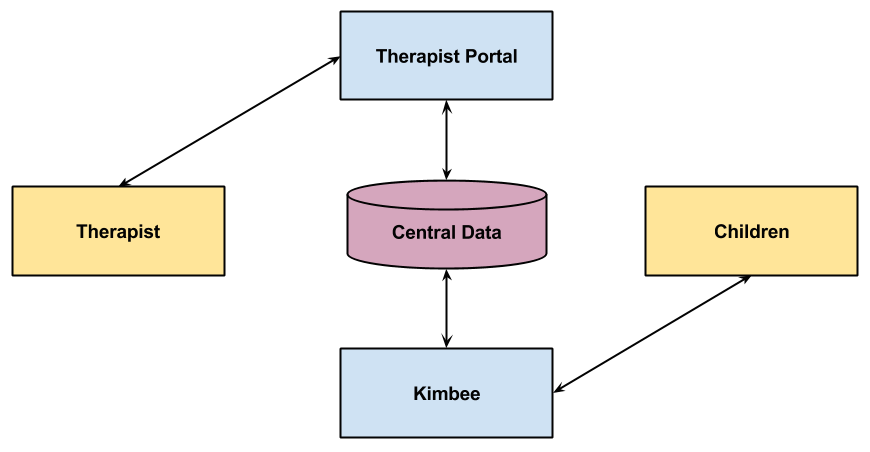
\includegraphics[keepaspectratio, width=\textwidth]{user_figure.png}
  \vspace{-22 pt}
  \caption{\normalfont Left: The game, {\em Kimbee}, where children play the role of a bee trying to collect honey as a resource. Right: The flow diagram showing how therapists and children exchange data through the game and the portal.}
  \label{fig:user}
\end{figure*}

\subsection{User Flow}

The flow is split into two parts, one to describe the game the child or user would play and another to describe what the therapist would see after the child has played the game. This will follow the example that the therapist has assigned {\em Kimbee} as homework for the child to do at home outside of the session. When the game is launched for the first time, a unique identification string is generated as a token for the child. This token should then be sent to the therapist allowing them to track the progress of the student. It is suggested that this first launch and setup take place in an in-person session with the therapist to alleviate any technical problems that may arise.

\subsubsection{Gameplay\label{sec:gameplay_flow}}

The game has a simple interface that is easy for a child to navigate, see Figure \ref{fig:user}. Children simply tap the screen to make their character, a bee, move along the y-axis of the screen. Collecting honey causes their score to increase and colliding with an enemy wasp causes the game to end. Interleaved with the enemy wasps and honey pots is a special honey pot that will grant a significant amount of honey if a challenge is completed. This challenge consists of having the child speak into the microphone of his or her device and say a designated word or phrase that appears on the screen.

The difficulty of the text increases over time to simulate the treatment that the child would receive during a therapist session \cite{Rosenbek:Treatment}. If the system succeeds in verifying that the child spoke the text correctly, then the currency is added to the child's score. If the child fails to correctly pronounce the phrase or if the system fails to recognize the audio, then the child is asked to try again in order to continue. To avoid discouraging the child, {\em Kimbee} will say a positive statement asking him or her to try again to continue playing the game.

After every challenge, the audio spoken by the child is encoded and sent to the central data server, see Figure \ref{fig:user} for a diagram of this. These data can be examined and reviewed in the therapist portal.

\subsubsection{Therapist Review}

The therapist is responsible for tailoring lesson plans for each session with his or her students. Currently, this involves taking detailed notes during every session to document and track the progress of each student over time \cite{Kreider:Intro}. The goal of the Therapist Portal is to improve and simplify this process to increase the quality of treatment given to the student. As described in section \ref{sec:gameplay_flow}, every recording that each child produces will be sent to the central server. These recordings are then sent to Therapist Portal and listed for every student under the therapist. Additional data is sent down with each recording to help the therapist focus on words that the student had trouble speaking. For example, whether the child said the word or phrase correctly is included with the recording allowing the therapist to filter the recordings.

After listening to all of the recordings that the child produced for homework, the therapist will have a good idea for where the student currently is in terms of progress. With this new information, the therapist will be able to start of the next in-person session with a more focused lesson plan.

\subsection{Currency}

As mentioned in section \ref{sec:related}, many other applications failed to create a captivating game for children. We wanted to have an application that children would see less as homework and more of a game. This was the underlying motivation for making {\em Kimbee} a game. In order for a game to be immersive, a sense of progression must be present \cite{Ermi:Gameplay}. We were able to create this using the honey collected as a currency. We also added the dynamic scoring of the honey, with the collection of the pots and completion of the challenges.

Many therapists currently use operant conditioning as a reward system \cite{Kreider:Intro}. For example, Kreider rewards children with small toys after they do well on a set of phrases. A reward system could be implemented where the currency is the honey from {\em Kimbee}. This would encourage students to play the game outside of the therapy sessions and motivate them to improve over time. As this was only a quarter long project, this is left as future work.\label{sec:currency}

\begin{figure*}[t]
  \centering
  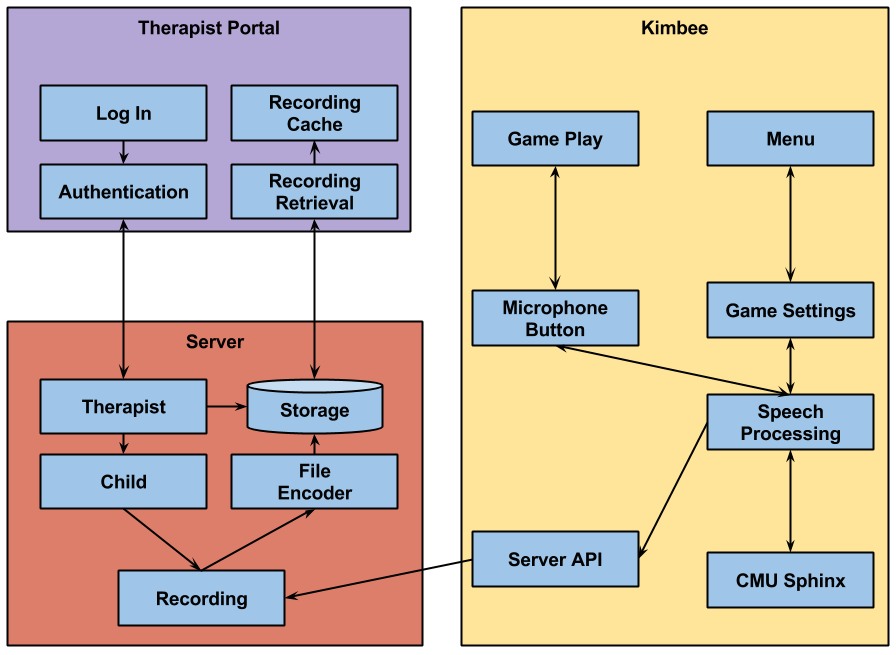
\includegraphics[keepaspectratio, width=\textwidth]{tech_figure.png}
  \vspace{-23 pt}
  \caption{\normalfont Left: The Therapist Portal, the user system of the therapist. Middle: The Central Server, hosts the recordings and facilitates interactions. Right: The Kimbee Game, interactive game that allows practice of speech for children. }
  \label{fig:tech}
\end{figure*}

\section{Implementation Details}

We will now discuss the implementation details of each of the systems that make up {\em Kimbee}. This project is made up of many components. In particular we will discuss the three main systems: the Server, the Game, and the Therapist Portal. From a high level, the Game and the Therapist Portal are thinly interconnected to the Server via HyperText Transfer Protocol (HTTP).

\subsection{Game ({\secit Kimbee})}
The {\em Game}, see Figure \ref{fig:tech}, is the system that the children interact with to practice speech. It is written in TypeScript and compiled to optimized JavaScript. Since this system also performs speech processing to determine speech correctness, there are many interacting components. From a high level, the major sub systems are: the {\em Phaser Game Implementation}, the {\em Speech Processing Component}, and the {\em Server Application Programming Interface (API)}. We target this project toward web technologies to allow wide distribution and adoption. From a design standpoint, we aimed to make each system loosely connected and non-disruptive to game-play. This required us to explore various new web technologies including HTML5 Web Workers for multi-threading and the UserMedia HTML5 API.

\subsubsection{Platform choice}
Since we want this project to work on as many devices as possible, we target emerging web technologies that work seamlessly across all devices with a web browser component. The web technology stack is advanced enough to handle our needs: there is a JavaScript port of the popular speech processing library CMU Sphinx, and we now have access to the user's microphone via UserMedia HTML5 API. After creating our project in the browser, we then can translate it to native applications via Apache Cordova, a web distribution technology based on embedding a web component inside a native application container on mobile devices.

\subsubsection{Phaser Game Implementation}
The {\em Phaser Game Implementation} of the {\em Game} encompasses the view and control of the application: The main menu, the game play, and rendering. This is what the children interact with to practice speech. The game is implemented with the Phaser Game Framework  which represents screens of the game into states. States are linked together in meaningful ways. For example, the Main Menu State links to the Option Menu State via a Phaser Framework Button. It also provides image animation, tweening, and collision support. To create our microphone button, we extend the Phaser Framework Button and implement connections to the speech processing component while preserving button functionality through inheritance.

\subsubsection{Speech Processing}
The {\em Speech Processing} of the {\em Game} handles all audio processing and speech related requests from the {\em Phaser Game Implementation}. Requests are made through an API Singleton that is constructed on game load. These include requests such as getting the next practice word for a particular speech problem, setting which speech problem the child is working on, and harvesting microphone data. Harvesting and processing microphone levels is a multi-threaded process implemented with HTML5 Web Workers. When the application is started and the API Singleton is constructed, audio stream {\em consumers} are created to process future audio streams in separate threads. Once a microphone ``Start'' request is made from the {\em Phaser Game Implementation}, the following steps are executed:
\vspace{-3 pt}
\begin{enumerate}
  \item Web Workers are initialized to start processing the audio stream in parallel.
  \vspace{-6 pt}
  \item Each stream buffer is processed by each Web Worker in parallel as the microphone streams raw Left-Right buffers.
  \vspace{-6 pt}
  \item Once a microphone ``Stop'' request is made from the {\em Phaser Game Implementation}, the consumers are queried for final results of their processing.
\end{enumerate}
\vspace{-3 pt}
Currently there are two {\em consumers}: an {\em AudioStorageConsumer}, and a {\em RecognizerConsumer}. The {\em AudioStorageConsumer} simply stores the raw microphone levels, while the {\em RecognizerConsumer} communicates with the {\em CMU Sphinx} to iterate a best guess for the correctness of the child's speech.

\subsubsection{CMU Sphinx}
CMU Sphinx is a speech processing library \cite{CMU:Sphinx}. There is a JavaScript port that allows audio recognition in the browser. Our {\em Speech Processing} component utilizes this JavaScript port to do audio recognition in the browser without server assistance. To deduce correct child speech we utilize this library creating target word and invalid word pairs. For example, when targeting `R' sounds, we can use CMU Sphinx to recognize the target word `Rabbit' or a invalid word `Wabbit.' With a large dictionary of words this has been effective in distinguishing replacements caused by speech disorders.

\subsubsection{Server API}
The {\em Server API} is what connects the {\em Game} to our central recording server. Once audio is processed by the {\em Speech Processing}, it is sent off via POST request in raw microphone form to the central server if a Internet connection is present. A unique identifier is computed and stored by the Kimbee System that will uniquely identify recordings in the central server as belonging to a particular child's device. This unique identifier is accessible via the Options Screen in the {\em Phaser Game Implementation}.

\subsection{Central Server}
The {\em Central Server}, see Figure \ref{fig:tech}, facilitates communication between all the {\em Game} instances and the {\em Therapist Portal}. It is written in Node JS and stores data in a MongoDB instance. We also do audio encoding to create playable audio files from child microphone data obtained from {\em Game} instances.

\subsubsection{Data Models}
The server has three data models: recordings, children, and therapists. Recordings are the microphone encodings and recognition data from the {\em Game} instances. They are tied to a particular game instance via a unique token generated by the {\em Game}. Children are models created by therapists to effectively ``hook into'' recordings. They specify a name for the child and their token obtained from their {\em Game} instance. Future recordings are then relayed to the therapist from this particular {\em Game} instance. Finally, therapists are the authenticated user records that contain a user email and password and provides access into the therapist portal.

\subsubsection{Audio Encoding \& Recording Storage}
When a audio file is received by a {\em Game} instance, we encode it into a WAV file by interleaving the left and right buffer channels from the microphone. This file is then compressed and stored into the database as a recording. The recognition data (whether the {\em Game} instance thinks the recording was correct) and the target word are also stored with the recording model.

\subsubsection{Therapist Portal API}
The server exposes a set of APIs for the {\em Therapist Portal} to utilize. This includes functionality to retrieve recordings for a particular child owned by the therapist record, retrieve the authenticated therapist record, authenticate therapists, and register therapists. This functionality is used via a HTTP interface with the {\em Central Server}.

\subsection{Therapist Portal}
The {\em Therapist Portal}, see Figure \ref{fig:tech}, is the application the therapist will use to track his or her student's progress and listen to the student's audio recordings. It is written in Javascript using the jQuery library with Bootstrap for the design elements and look of the page.

\subsubsection{Connection to Child Audio}
When the portal is launched, the data for all of the children under the therapist is downloaded through a HTTP GET request to the central server. The data is returned as a JSON object a short amount of time after the page is loaded. The WAV files for each recording are not downloaded at this time because of the significant size of each file. Instead, each recording is lazy instantiated and only requested when the user clicks play. A unique ID represents each audio recording and if clicked, a request will be made to the central server for the WAV file of the recording. When this request returns with the audio, the data is injected into the DOM through a HTML audio tag and then played.

\subsubsection{Caching System}

Before any request for a recording is made, a cache is first checked to see if the recording is already on the client. If a cache miss occurs, then the request will be made. If a cache hit occurs, then the audio will be immediately injected into the DOM and played. This system allows the therapist to replay the same audio recording multiple times without having to make a significant number of requests. A system for pre-fetching was discussed but never implemented; we leave this as future work.

\section{Results}

Upon the completion of {\em Kimbee}, we met with Kreider in order to assess how a professional speech therapist would respond to the application and to see if he had any suggestions and improvements \cite{Kreider:Results}. His reaction was very positive. He found no real flaws with the application and expressed that it would be very useful for children to work with. He wants us to continue consulting and working with him in the future as he thought that {\em Kimbee} was very promising. He did have suggestions for the future that are listed below under section \ref{sec:future_work}. Unfortunately we did not have time to test our application with actual children and track the results but we are confident that {\em Kimbee} can be used in a real world setting.

\section{Future Work}
\label{sec:future_work}

There are a few ways that we can expand on {\em Kimbee}. We plan on deploying the project for use in the Arlington Public School District to see how children respond and learn from {\em Kimbee} along with how experienced speech therapists use {\em Kimbee} to aid the therapy process. Along with this, we can also expand on the application itself by targeting speech sounds past the `R' and `W' sound replacement. We can also enhance the child's experience by adding more mini-games for the child to play and a token system for children to spend the honey they collect on aesthetics for the bee character. The token and currency system described at the end of section \ref{sec:currency} is also left as future work.

\section{Conclusion}

{\em Kimbee} is an application which uses speech recognition to help children and speech therapists better remedy speech impediments. While it currently only focuses on `R' to `W' sounds, it can be further expanded to supplement therapy by giving a therapist the recordings of a child in a remote setting and by giving a child the opportunity to practice more than the short time period allotted weekly. By giving children an enjoyable speech therapy tool we hope to save the money of both schools and parents while simultaneously giving children a better education by helping them overcome their speech impediment as quickly as possible.

\section{Acknowledgments}

We would like to thank Richard Kreider of the Arlington Public School District for meeting with us to discuss the viability and details of our project when it was in its developing stages and then again to discuss improvements when Kimbee was almost finished \cite{Kreider:Intro,Kreider:Results}. We would also like to thank Bruce Hemingway and Hanchuan Li for helping us throughout the project with guidance and feedback.

\bibliographystyle{abbrv}
\bibliography{sigproc}

\balancecolumns

\end{document}
